% Suggested Viewer : Okular 4.8.5
\documentclass[xcolor=dvipsnames]{beamer}

\usepackage[utf8]{inputenc} 
\usepackage[T1]{fontenc}
\usepackage{lmodern}
\usepackage{graphicx}
\usepackage{multimedia}
\usepackage{tikz}
\usepackage[]{algorithm2e}
%compatible for older versions
\providecommand{\SetAlgoLined}{\SetLine}

\usetheme{Warsaw}

%\graphicspath{...}


\definecolor{UniOrange}{RGB}{146,28,80}
\definecolor{UniFont}{RGB}{255,255,255}
\definecolor{UniViolet}{RGB}{92,30,86}
\setbeamercolor*{palette primary}{use=structure,fg=UniFont,bg=UniViolet}
\setbeamercolor*{palette quaternary}{fg=UniFont,bg=UniOrange}
\setbeamercolor{structure}{fg=UniViolet,bg=UniViolet}

\defbeamertemplate*{footline}{shadow theme}
{%
  \leavevmode%
  \hbox{\hskip-0.05ex
    \begin{beamercolorbox}[wd=.45\paperwidth,ht=2.5ex,dp=1.125ex,leftskip=.3cm plus1fil,rightskip=.3cm]{author in head/foot}%
      \usebeamerfont{author in head/foot}\hfill\insertshortauthor
    \end{beamercolorbox}%
    \begin{beamercolorbox}[wd=.45\paperwidth,ht=2.5ex,dp=1.125ex,leftskip=.3cm,rightskip=.3cm plus1fil]{title in head/foot}%
      \usebeamerfont{title in head/foot}\insertshorttitle%
    \end{beamercolorbox}%
    \begin{beamercolorbox}[wd=.11\paperwidth,ht=2.5ex,dp=1.125ex,leftskip=.3cm,rightskip=.3cm plus1fil]{author in head/foot}%
      \usebeamerfont{author in head/foot}\insertframenumber\,/\,\inserttotalframenumber%
    \end{beamercolorbox}
  }%end of hbox
  \vskip0pt%
}

\setbeamertemplate{navigation symbols}{}

% re-definition of the title page
\setbeamertemplate{title page}{
\centering
\begin{beamercolorbox}[rounded=true,shadow=true,sep=8pt,center]{title}
\inserttitle \par
\end{beamercolorbox}
\vfill
{\small \em
  Ma Jun and Ma Shaoan\\
  Journal of Computer Science and Technology\\
}
\vfill
\centering
\begin{columns}[T]
  \begin{column} {.05\textwidth}
  \end{column}
  \begin{column} {.3\textwidth}
  {\em Students:}\\
  \tiny
  \insertauthor
  \end{column}
  \begin{column} {.34\textwidth}
  \end{column}
  \begin{column} {.3\textwidth}
  {\em Supervisors:}\\
  \tiny
  \supervisors
  \end{column}
\end{columns}
\vfill
\usebeamerfont{institute}\insertinstitute \par
\vfill
\centering
\presentationdate\par
\vfill
}


\AtBeginSection[]
{
\begin{frame}
	\tableofcontents[currentsection, hideothersubsections]
\end{frame}
}

%TODO better title
\title[$O(k^2n^2)$ algorithm for $k$-partitionning]{Study of the article :\\``An $O(k^2n^2)$ algorithm for $k$-partition in a $k$-connected Graph''}

\author[Lambert, Gharsalli, Hofer]
       {Thibaud Lambert\\Mohammed Ayoub Gharsalli\\Ludovic Hofer}

%TODO separate content and form supervisors
\newcommand{\supervisors}{Olivier Baudon\\Julien Bensmail\\Pascal Desbarats}

\newcommand{\presentationdate}{
  December ... 2013
}

\institute{University of Bordeaux I}

\begin{document}

\begin{frame}[plain]
  \maketitle
\end{frame}

\begin{frame}[plain]
  \tableofcontents
\end{frame}

\section{About Graphs}

\begin{frame}
  \frametitle{Graph Theory}
  \begin{itemize}
  \item Powerful tool for modeling
    \begin{itemize}
    \item relations
    \item processes
    \end{itemize}
  \item Examples
    \begin{description}
     \item [Social network:] Node: person, Edge: friendship relation
     \item [Neuroscience:] Modeling neural network  \cite{BuSp09}
     \item [Telecommunications:] Peer-to-peer mobile networks  \cite{FaCh99}
    \end{description}
  \end{itemize}
\end{frame}

\begin{frame}
  \frametitle{Undirected simple Graphs}
  \begin{itemize}
    \item Formal Description
      \begin{itemize}
      \item $G = (V,E)$
      \item $V$ an unordered set of vertex
      \item $E$ an unordered set of unorder pairs $(u,v), u \in V, v \in V$
      \end{itemize}
    \item {\em Example picture coming soon...} % TODO Ayoub
  \end{itemize}
\end{frame}

\section{Problem Description}

\begin{frame}
  \frametitle{$k$-connected graphs}
  \begin{itemize}
    \item $G$ is $k$-connected $\Leftrightarrow \forall (u,v) \in V^2$
      \begin{itemize}
      \item At least $k$ edge-disjoint paths from $u$ to $v$
      \end{itemize}
    \item path of length $n$ : $\{v_0,e_1,v_1,e_2, \dots , e_n,v_n\}$
    \item $P_1$ edge-disjoint to $P_2$ : no edges shared
  \end{itemize}
  \begin{figure}
  \begin{center}
    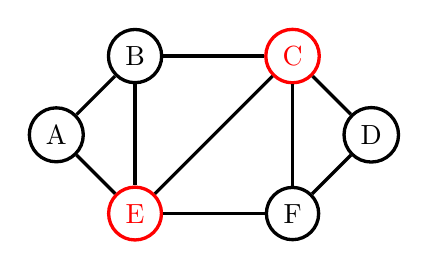
\begin{tikzpicture}[scale=0.5]
  \node[draw,circle, very thick] (A) at (0,2) {A};
  \node[draw,circle, very thick] (B) at (2,4) {B};
  \node[draw,circle, very thick, color=red] (C) at (6,4) {C};
  \node[draw,circle, very thick] (D) at (8,2) {D};
  \node[draw,circle, very thick, color=red] (E) at (2,0) {E};
  \node[draw,circle, very thick] (F) at (6,0) {F};
  \draw[very thick] (A) -- (B);
  \draw[very thick] (A) -- (E);
  \draw[very thick] (B) -- (C);
  \draw[very thick] (B) -- (E);
  \draw[very thick] (C) -- (D);
  \draw[very thick] (C) -- (E);
  \draw[very thick] (C) -- (F);
  \draw[very thick] (D) -- (F);
  \draw[very thick] (E) -- (F);
\end{tikzpicture}

    \end{center}
    \caption{A 2-connected graph}
    \end{figure}
\end{frame}

\begin{frame}
  \frametitle{$k$-partition}
  \begin{itemize}
  \item Obtain $\{V_1, \dots, V_k\}$ with
    \begin{itemize}
    \item $\forall i, \lceil V_i \rceil$ is connected
    \item $\sum\limits_{i=0}^k|V_i| = |V|$
    \item $\forall i,j \in \{1, \dots, k\}^2, i \neq j, V_i \cap V_j = \emptyset$
    \end{itemize}
  \end{itemize}
  \begin{center}
    
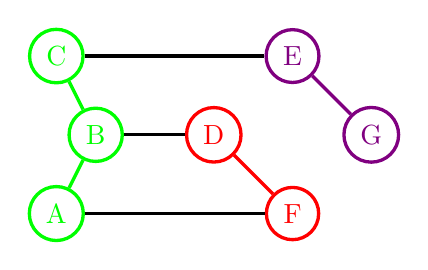
\begin{tikzpicture}[scale=0.5]
  \node[draw,circle, very thick, color=green] (A) at (0,0) {A};
  \node[draw,circle, very thick, color=green] (B) at (1,2) {B};
  \node[draw,circle, very thick, color=green] (C) at (0,4) {C};
  \node[draw,circle, very thick, color=red] (D) at (4,2) {D};
  \node[draw,circle, very thick, color=violet] (E) at (6,4) {E};
  \node[draw,circle, very thick, color=red] (F) at (6,0) {F};
  \node[draw,circle, very thick, color=violet] (G) at (8,2) {G};
  \draw[color=green, very thick] (A) -- (B);
  \draw[color=green, very thick] (B) -- (C);
  \draw[very thick] (B) -- (D);
  \draw[very thick] (A) -- (F);
  \draw[very thick] (C) -- (E);
  \draw[very thick, color=violet] (E) -- (G);
  \draw[very thick, color=red] (D) -- (F);
\end{tikzpicture}

  \end{center}
\end{frame}

\begin{frame}
  \frametitle{Article Description}
  \begin{itemize}
  \item Finding a $k$-partition
    \begin{itemize}
    \item In a $k$-connected graph
    \item Choosing $k$ vertices $\{a_1, \dots , a_k\}$
    \item Choosing the size of each component $\{n_1, \dots ,n_k\}$,
      $\sum\limits_{i}^k{n_i} = n$
    \item Complexity : $O(k^2 n^2)$
    \end{itemize}
  \item Published in {\em ``Journal of computer science and technology''}
    \begin{itemize}
    \item National Journal
    \item Bimonthly published
    \end{itemize}
  \end{itemize}
\end{frame}

\section{State of art}

\begin{frame}
  \frametitle{Finding the $k$-connectivity of a graph}
  \begin{itemize}
  \item  Link between :
    \begin{itemize}
    \item $k$-connectivity 
    \item Minimum vertex cut size
    \item Maximum, flow (Max-flow min-cut theorem)
    \end{itemize}

  \item Algorithm
    \begin{itemize}
    \item Compute maximum flow with vertex unitary capacity
    \item Deduce the $k$-connectivity
    \end{itemize}
  \end{itemize}

\end{frame}

\begin{frame}
  \frametitle{$k$-partition of $k$-connected graphs}
  \begin{itemize}
  \item According to the article
    \begin{itemize}
    \item For a general graph $G$, finding a $k$-partition is a $NP$-hard
      problem\cite{Dyer1985139}
    \item If $G$ is a $k$-connected graph, a $k$ partition exists\cite{GE78,LL77}
    \item Polynomial solutions for $k = 2$\cite{GE78,LL77} and
      $k = 3$%citation needed
    \item No general polynomial algorithms found
    \end{itemize}
  \item Now
    \begin{itemize}
    \item linear algorithm for $k = 4$\cite{Nakano1997315}
    \end{itemize}
  \end{itemize}
\end{frame}

\section{Work needed}

\begin{frame}
  \frametitle{Validation of the algorithm}
  \begin{itemize}
  \item Major breakthrough but very few citations
  \item Tested, but on what graphs?
  \item Verifying the algorithm validity and complexity
    \begin{itemize}
    \item By understanding it
    \item By implementing it
    \end{itemize}
  \end{itemize}
\end{frame}

%\begin{frame}
%  \frametitle{Generating $k$-connected graphs}
%  \begin{itemize}
%    \item Random $k$-connected graph uniform generation
%      \begin{itemize}
%      \item Difficult problem
%      \end{itemize}
%    \item Trails to explore
%      \begin{itemize}
%      \item Generate complete sub-graph and link them together
%      \item Generate a graph with all vertices of degree $k$
%      \end{itemize}
%  \end{itemize}
%
%\end{frame}
%
%\begin{frame}
%  \frametitle{Pre-processing algorithm}
%  \begin{itemize}
%  \item Original complexity in $O(k n m)$
%  \item Existing algorithm to induce a spanning subgraph\cite{NaIb92}
%    \begin{itemize}
%    \item $G' = (V,E')$
%    \item $|E'| = O(k n)$
%    \item Complexity of the algorithm : $O(m)$
%    \end{itemize}
%  \item Implementation needed to get the $O(k^2 n^2)$ complexity
%  \end{itemize}
%\end{frame}
%
%\begin{frame}
%  \frametitle{Algorithm implementation}
%  Different parts of the algorithm
%  	\begin{enumerate}
%    \item Graph Sparsing
%	\item Graph Partitionning
%    \end{enumerate}
%	
%	{\bfseries Graph partitionning}\\
%    	 \begin{description}
%		\item [INPUT:] \hfill \\
%		        \begin{enumerate}
%        			\item $G = (V, E)$ a $k$-connected graph 
%            		\item $k$
%            		\item $a_1, a_2 \ldots a_k$ : different vertices of $G$
%            		\item $n_1, n_2 \ldots n_k$ : strictly positive integers of $\sum_i n_i =  V(G)$
%        		       \end{enumerate}
%	\end{description}
%\end{frame}
%\begin{frame}
%    	 \begin{description}
%		\item[OUTPUT:] \hfill \\
%			A k-partition $Par$ of G such that $\forall i \ in 1..k$ 
%			\begin{itemize} 
%				\item $H_i$ is a connexe subgraph of $G$
%				\item $H_i \in Par, |V(H_i)| = n_i $
%				\item $a_i \in H_i $
%				\item $\forall j \in 1..k H_i \bigcap H_j = \emptyset$
%			\end{itemize}
%	\end{description}
%\end{frame}
%
%\begin{frame}
%	\begin{description}
%    	\item[Definitions] \hfill \\
%    	\begin{itemize}
%    		\item [$T_i$] a spanning tree which root is $a_i$.
%			\item[P] \hfill \\
%    		The proposed algorithm is similar to \emph{max flow} algorithms.
%	 		$\forall i \in 1..k,$ \bfseries P $: T_i \rightarrow n_i/|V(T_i)|$
%		\item [$n$] $= |V(G)|$
%    	\end{itemize}
%    \end{description}
%\end{frame}
%
%\begin{frame}
%	\begin{algorithm}[H]
%    \SetAlgoLined
%    Initialisation\;
%		\While {$\sum_i |T_i| < n$}{
%			\While {$|T_i| < n_i$}{
%        		Add random adjacent vertices to $T_i$\;}
%		$T_i$ := the tree with highest $P$\;
%            	 $T_j$ := the tree with highest $P$ among adjacent trees to $T_i$\;
%		$U^{ij}_{adjacent}$ := the part of $T_j$ adjacent  to $T_i$\;
%		$w$	:= $max_{degree(v)} v \in T_j \bigcap  U^{ij}_{adjacent}$\;
%		Remove the subtree which root is $w$ from $T_j$\;
%		Add $w$ to $T_i$\;}
%	\end{algorithm}
%\end{frame}


\begin{frame}
\frametitle{Implementation}
\begin{description}
	\item [Objectives :] \hfill \\
	\begin{itemize}
		 \item Allow testing 
		\item Observe and measure performance
        \item verify consistency with complexity
     \end{itemize}

 \item[Tools :] \hfill \\
		Java using Graph Library created at Labri
  \end{description}
\end{frame}

\begin{frame}{Implementation}
  \begin{itemize}
  \item Generating random $k$-connected graphs
  \item Pre-processing graphs
  \item Algorithm implementation
  \end{itemize}
\end{frame}

\begin{frame}
  \frametitle{Comparing results and theory}
  \begin{itemize}
  \item Comparing the result of the implemented algorithm
    \begin{itemize}
    \item With different $k$ for the same $n$
    \item With different $n$ for the same $k$
    \item With different $m$ for the same $n$
    \end{itemize}
  \item Comparing the execution time for different graph generators
  \end{itemize}
\end{frame}

\section*{References}
\begin{frame}[allowframebreaks]
  \frametitle{References}
  \bibliographystyle{amsalpha}

  \bibliography{bibliography}
\end{frame}

\end{document}
